\documentclass[12pt,notitlepage]{article}
\usepackage{draft}
\pdfoutput=1

\usepackage{tabularx}
\usepackage{latexsym}
\usepackage{ifthen}
\usepackage{epsfig}
\usepackage{graphics}
\usepackage{natbib}
\usepackage{amsmath}
\usepackage{amsfonts}
\usepackage{amssymb}
%\usepackage{amsthm}
\usepackage{algpseudocode}
\usepackage{algorithm}
\usepackage[margin=1in]{geometry}
\usepackage[hang,footnotesize,bf]{caption}
\usepackage{color,array}
\usepackage{hyperref}
\usepackage{bbm}	
\usepackage{mathtools}

\DeclarePairedDelimiter\ceil{\lceil}{\rceil}
\DeclarePairedDelimiter\floor{\lfloor}{\rfloor}
\definecolor{darkgreen}{rgb}{0,0.5,0}
\definecolor{darkblue}{rgb}{0,0,0.8}
\hypersetup{colorlinks, urlcolor=darkblue, citecolor=darkgreen}

\newcommand{\makecell}[2][@{}c@{}]{\begin{tabular}{#1}#2\end{tabular}}

\begin{document}

%
\title{{\bf Slow journey to racial diversity: Florida Story}}
%
\author{
  Gaurav Sood\thanks{
  Email: gsood07@gmail.com} \\
\and
  Seung Lee\thanks{
  Email: slee126@ucsc.edu} \\
}
%
\date{\today}

\renewcommand{\baselinestretch}{1}
\maketitle

\renewcommand{\baselinestretch}{1}
\selectfont
%
\begin{center}
{\bf Abstract}
\end{center}
%
\par
\begin{footnotesize}
  \begin{quote}
We analyze Florida
    \\[2ex] 
  \end{quote}
\end{footnotesize}
%
\textbf{Keywords:} Race Diveristy, Race Impute \newpage

\renewcommand{\baselinestretch}{1.5}

\selectfont
\section{Data}
\label{intro}



We combine university, state, city,  county, and k-12 school teacher's payroll data.  Each institution's payroll data has amount paid to an individual's name i.e. John Smith \$15000.  We run the names through 4 algorithms that impute race using an individual's first and/or last name.  We use \href{https://github.com/appeler/ethnicolr}{Ethnicor}'s algorithms, which uses US census data and Florida voting registration data to determine the race of an individual.  We average the 4 algorithms' predictions for our analysis.  

%
\section{Analysis}

\label{intro}

\subsection{Race Composition Across Institutions}
Comparing the  \href{https://en.wikipedia.org/wiki/Demographics_of_Florida}{2010 census}  and \href{https://www.census.gov/prod/2002pubs/c2kprof00-fl.pdf}{2000 census} we find 
White-Not Hispanic race proportion dropped from 60\% to 53.5\%, 11\% drop in 10 years.  The white-not Hispanic race proportion in (university, state, city, school teachers, county) has only dropped 4-6\% in the years spanning longer than that period.  Florida public payroll data shows all race is under-represented across (university, state, city, school teachers, county) except for Asians at the university level, which only constitutes 8\% of Florida's public payroll data counts.


\begin{figure}[H]
\begin{center}
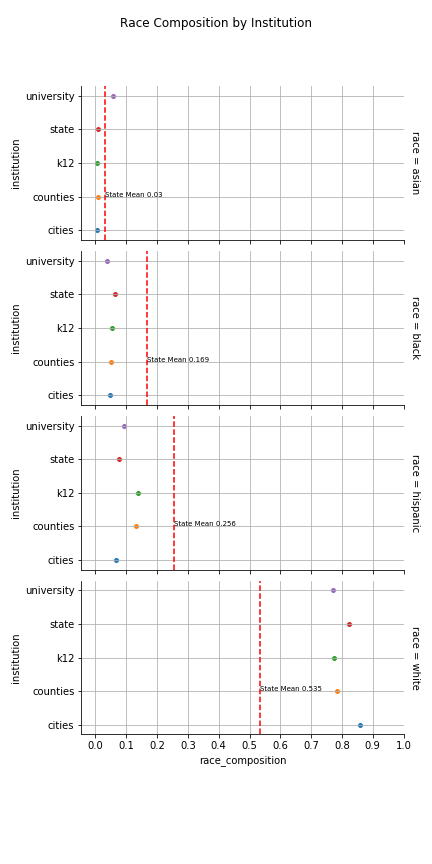
\includegraphics[width=3.5in]{Figures/race_composition_across_inst.png}
\caption{Florida's public sector race composition}
\label{styleResponse}
\end{center}
\end{figure}


\subsection{Institution median pay by race}
fill in


\begin{figure}[H]
\begin{center}
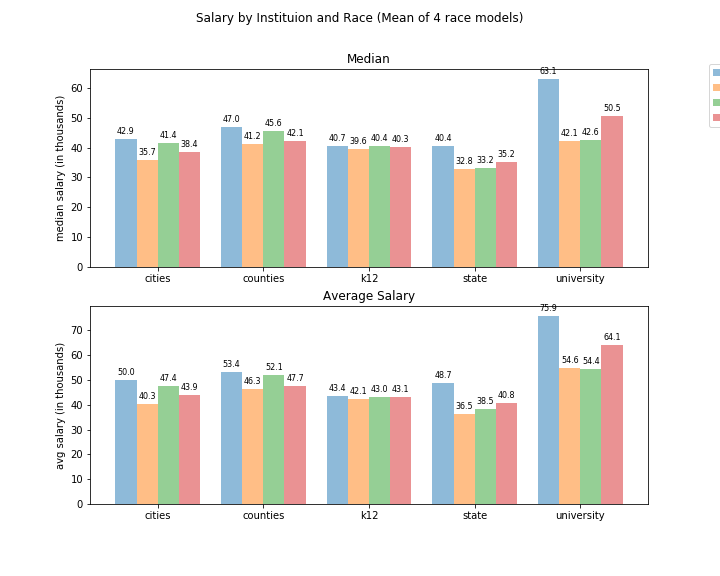
\includegraphics[width=5.5in]{Figures/race_median_pay}
\caption{Median pay of Florida's public sector by race }
\label{styleResponse}
\end{center}
\end{figure}

\subsection{Race Composition Time Series}
fill in


\begin{figure}[H]
\begin{center}
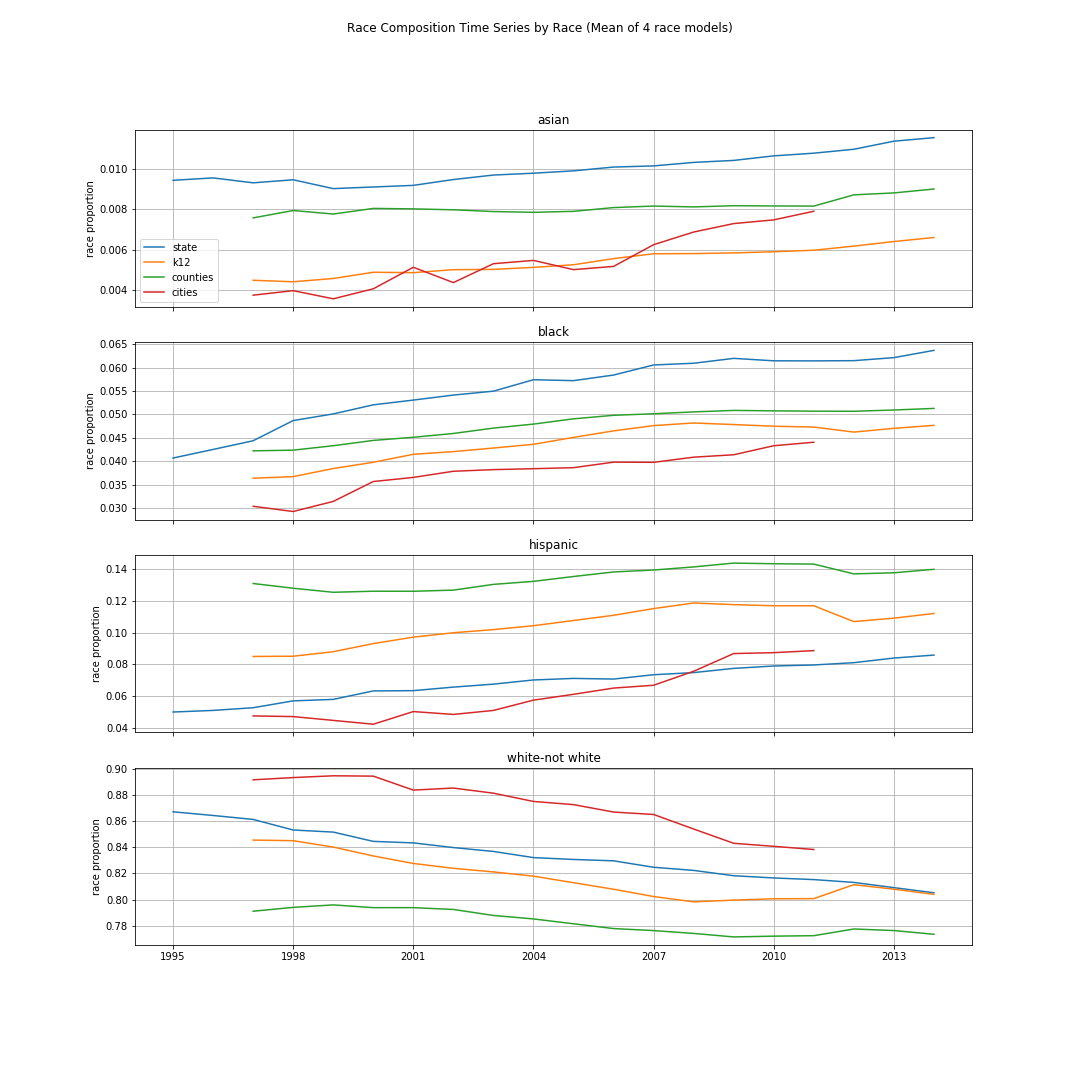
\includegraphics[width=5.5in]{Figures/race_composition_ts.png}
\caption{Time Series: Florida's public sector race composition}
\label{styleResponse}
\end{center}
\end{figure}


\subsection{Race Median Pay Time Series}
fill in


\begin{figure}[H]
\begin{center}
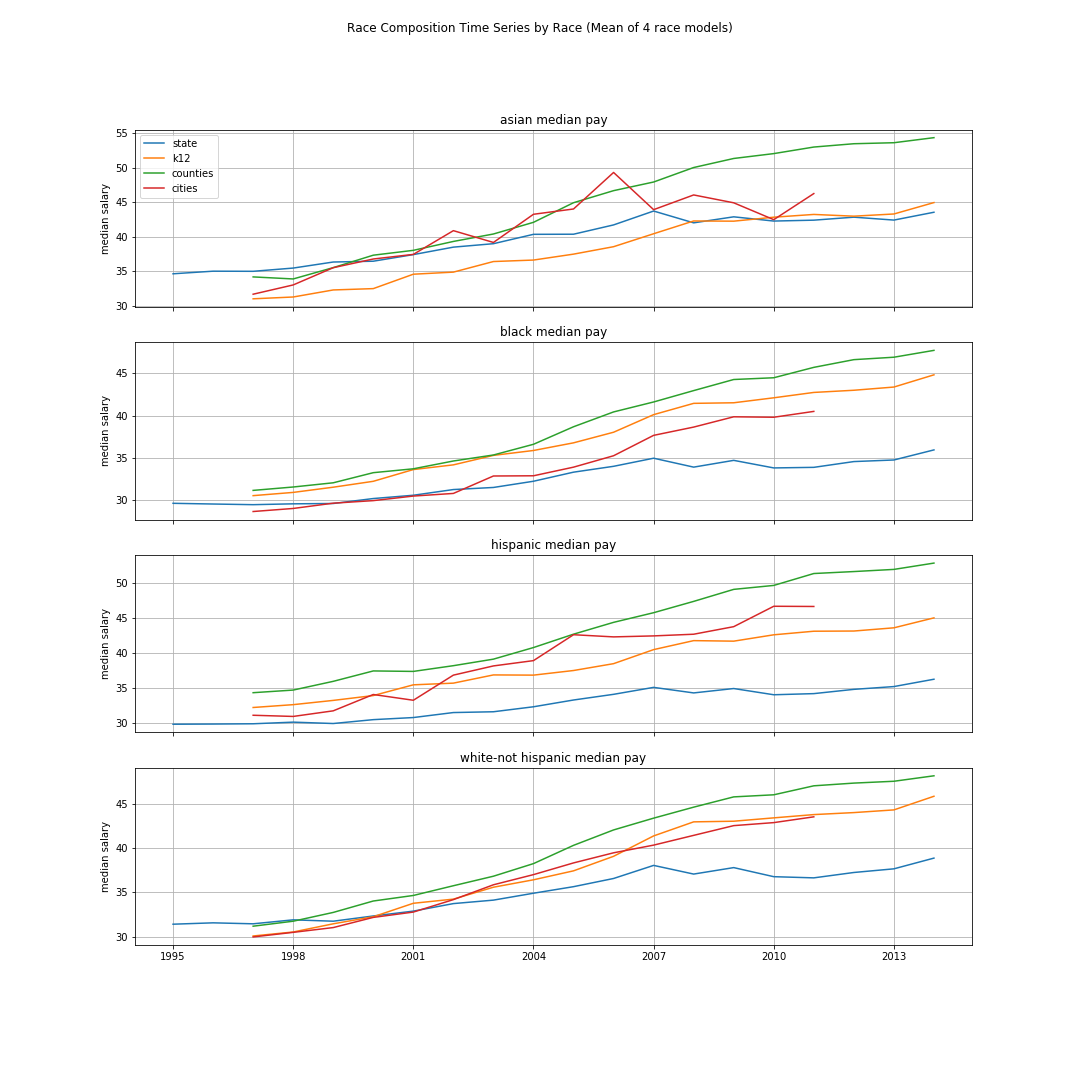
\includegraphics[width=5.5in]{Figures/median_salary_ts.png}
\caption{Time Series: Florida's public sector median pay}
\label{styleResponse}
\end{center}
\end{figure}%

%
%
%
\newpage

\renewcommand{\baselinestretch}{1}
\selectfont
\nocite{*}
\bibliographystyle{asa}


\end{document}


